\documentclass[a4paper,12pt]{article}
% \usepackage{multicol}  
\usepackage{graphicx} 
\usepackage{hyperref}
\usepackage{float}

\begin{document}

\title{Assignemnt 1 - Amazon Sales Analysis}
\author{Mohammad Hossein Basoulii}
\date{\today}
\maketitle

% \onecolumn
\begin{center}
    \section*{\textit{Abstract}}
    \textit{In this study we focus on a sales dataset gathered from \textbf{Amazon}. 
    By this, we are looking towards finding patterns and relationships between different factors in our dataset and their contribution to our sales. 
    We have used Exploratory Data Analysis (EDA) to get initial insights and form hypotheses about the data. 
    And then, we used statistical testing as a tool for testing our hypotheses. 
    Some of the key findings of this study showcase a independence of \textbf{discount price} and \textbf{ratings}, 
    dependence of \textbf{product category} and \textbf{ratings} and non-normality of \textbf{rating counts} for different products.}
\end{center}

% \begin{multicols}{2}

\section*{Introduction}
\textbf{Background}: Analysis of sales' data of e-commerce businesses has been a matter of great interest, since the very beginning of this era, for all of the companies which care about growing their benefit from the continuous change of demands that cutomers have over time. So the importance of this study is obvious. \\

\noindent\textbf{Objective}: We first, start off by forming some hypotheses about our data, e.g., does \textbf{discount price} affect \textbf{rating}?.  Then we try to find the correct way to test our hypotheses through Exploratory Data Analysis (EDA) section. And at the end, we actually go for Hypothesis Testing section, which would allow us to formally justify our hypotheses or reject them. \\

\noindent\textbf{Initial hypotheses}:
\begin{itemize}
    \item Does the discounted price significantly impact product ratings?
    \item Are product categories and high/low ratings independent?
    \item Is there a significant difference in ratings between high-discount and low-discount products?
    \item Do more expensive products receive higher ratings on average?
    \item Does the distribution of rating counts follow a normal distribution?
\end{itemize}

\section*{Data}
\textbf{Data Source}: The dataset comes from a sales' product record from \textbf{Amazon}. It has 1465 rows(sale records) and 16 different columns(features). \\

\noindent\textbf{Features}: numerical features include \textbf{discounted\_price}, \textbf{actual\_price}, \textbf{discount\_percentage}, \textbf{rating} and \textbf{rating\_count}.  The only important categorical feature is \textbf{category}. \\ 

\noindent\textbf{Data Preprocessing}: We find out that there is only two rows that have missing values. More specifically, these rows are missing values only on their \textbf{rating\_count} column.  We decide to just drop these rows, simply because missing them is insignificant, compared to the magnitude of the entire dataset.  We also need to apply a simple transformation to clean the data in columns \textbf{discounted}, \textbf{actual\_price}, \textbf{discount\_percentage}, \textbf{rating} and \textbf{rating\_count} and convert their initial data type to numeric to be able to work with them.


\section*{Exploratory Data Analysis(EDA):}
\subsection*{Univeriate Analysis:}
\textbf{Distributions of discounted\_price and rating}: \\

\noindent\textbf{Analysis}: By looking at the Figure~\ref{fig:Figure_1}, we can see that the distribution of both variables is skewed. Thus performing \textit{\textbf{Pearson Correlation Test}} wouldn't be appropriate for examining the relationship between these two variables, since assumption of normality of the variables is violated. \\

\noindent\textbf{Relevance}: This analysis would be importatnt when we want to decide whether if there is a relationship between these two variables. \\

\begin{figure}[H]
    \centering
    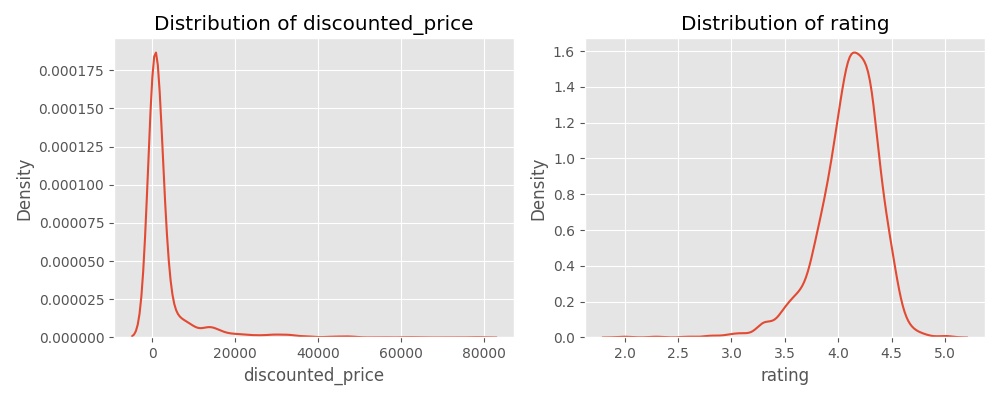
\includegraphics[width=0.8\textwidth]{./images/distro_of_discount_price_and_rating.png} % Change the filename and path
    \caption{Distributions of \textbf{discounted\_price} and \textbf{rating}}
    \label{fig:Figure_1}
\end{figure}

\noindent\textbf{Distribution of actual\_price}: \\

\noindent\textbf{Analysis}: By looking at Figure~\ref{fig:Figure_2}, we find out that distribution of \textbf{actual\_price} is skewed highly skewed as well. This could tell us that this variable is not normally distributed. \\

\noindent\textbf{Relevance}: This analysis would be important when we want to decide on what range of prices are low, medium and high later. \\ 

\begin{figure}[H]
    \centering
    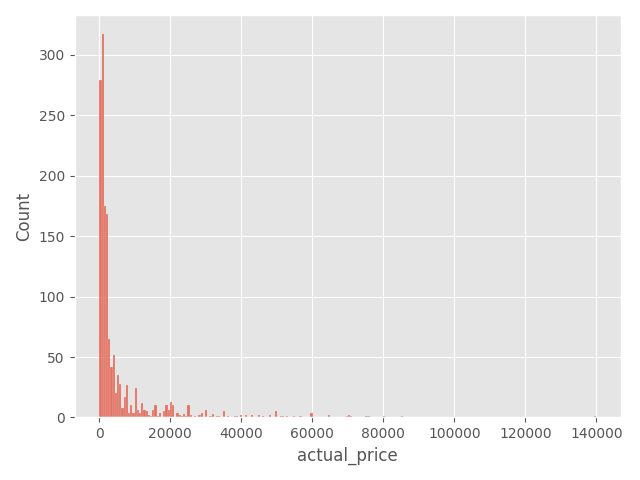
\includegraphics[width=0.8\textwidth]{./images/distro_of_actual_price.png} % Change the filename and path
    \caption{Distribution of \textbf{actual\_price}}
    \label{fig:Figure_2}
\end{figure}

\noindent\textbf{Distribution of rating\_count}:

\noindent\textbf{Analysis}: By looking at Figure~\ref{fig:Figure_3}, we find out that this variable is highly skewed to the right. Meaning that \textbf{rating\_count} of distinct products is not normally distributed. \\

\noindent\textbf{Relevance}: This analysis would be important when we want to test our hypothesis about the normality of this variable.\\

\begin{figure}[H]
    \centering
    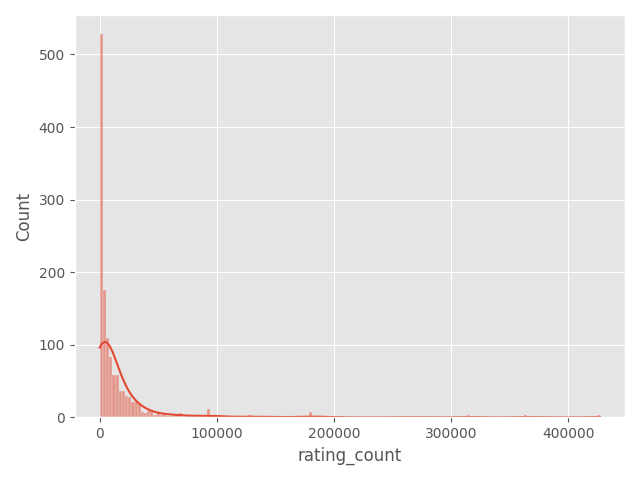
\includegraphics[width=0.8\textwidth]{./images/distribution_of_rating_count_for_products.png} % Change the filename and path
    \caption{Distribution of \textbf{rating\_count} for distinct products}
    \label{fig:Figure_3}
\end{figure}


\subsection*{Multivariate Analysis:}

\noindent\textbf{Scatter plot of discounted\_price and rating}:

\noindent\textbf{Analysis}: By looking at Figure~\ref{fig:Figure_4}, we figure out that there doesn't seem to be any monotonic relationship between these two variables. Thus we say that these two variables are uncorrelated. \\

\noindent\textbf{Relevance}: This analysis is connected with our prior Univeriate analysis about the distribution these two variables and would be investigated further in Hypothesis Testing section as well. \\

\begin{figure}[H]
    \centering
    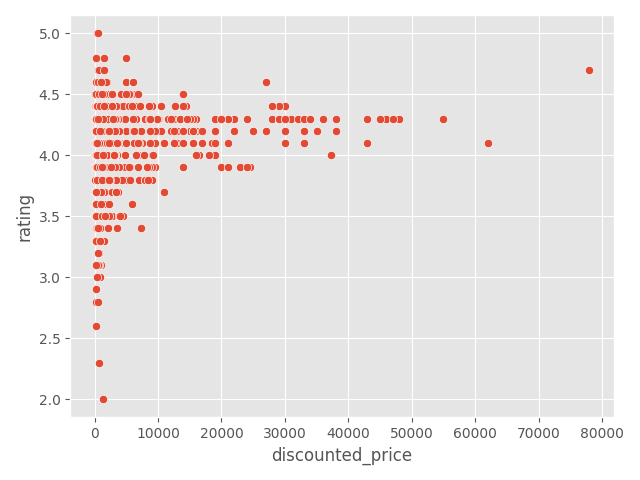
\includegraphics[width=0.8\textwidth]{./images/scatter_discounted_price_vs_rating.png} % Change the filename and path
    \caption{Scatter Plot of \textbf{discounted\_price} and \textbf{rating}}
    \label{fig:Figure_4}
\end{figure}

\noindent\textbf{Contingency Table of rating vs. category}:

\noindent\textbf{Analysis}: By Looking at Figure~\ref{fig:Figure_5}, we find out that there are some \textbf{categories}, which are different from others in terms of distribution of \textbf{rating\_levels}, namely, low and high. This could tell us that \textbf{category} and \textbf{rating} are dependent. \\ 

\noindent\textbf{Considerations}: We have dropped the records which are in a product \textbf{category} that has appeared less than 5 times in our entire dataset. This has been done, simple because the anaylsis of \textbf{rating\_level} within these groups would be totally meaningless because of their low frequency of appearance. \\ 

\noindent\textbf{Relevance}: This analysis would be used as an evidence to our future hypothesis testings of examining the dependence of these two variables.\\

\begin{figure}[H]
    \centering
    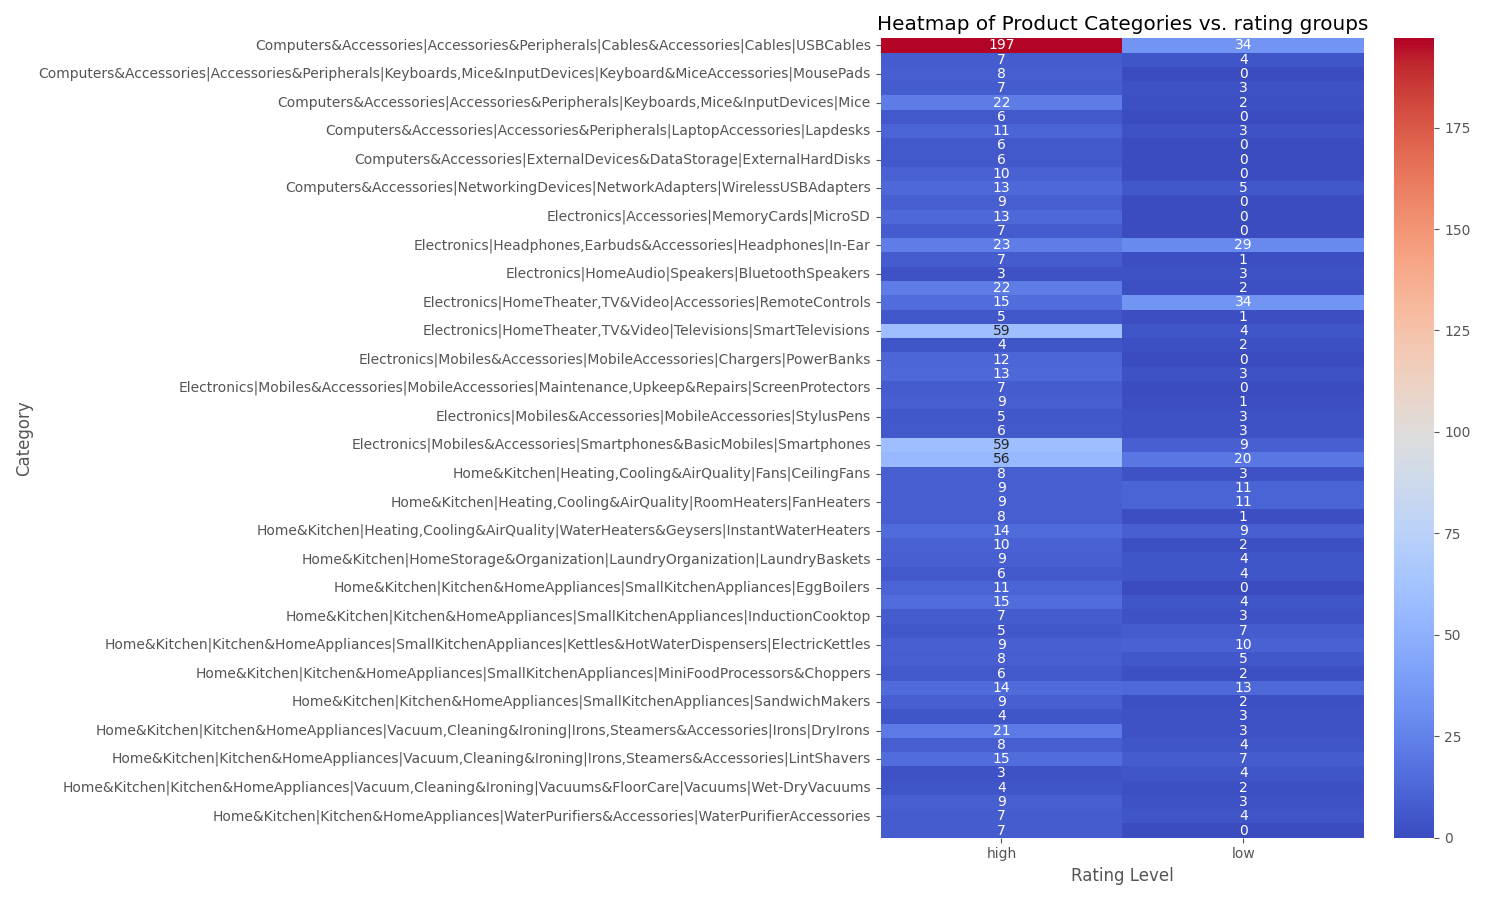
\includegraphics[width=0.8\textwidth]{./images/contingency_category_rating.png} % Change the filename and path
    \caption{Contingency Table of \textbf{category} and \textbf{rating\_level}}
    \label{fig:Figure_5}
\end{figure}

\noindent\textbf{Distribution of rating for low/high discount\_percentages}:

\noindent\textbf{Analysis}: By looking at Figure~\ref{fig:Figure_6}, we figure out that there doesn't seem to be a significant difference between the means of these two levels of \textbf{discount\_percentage} in terms of \textbf{rating}. \\ 

\noindent\textbf{Relevance}: This analysis would be used in hypothesis testing section, when we want to examine, more formally the difference between these two levels of \textbf{discount\_percentage}. \\

\begin{figure}[H]
    \centering
    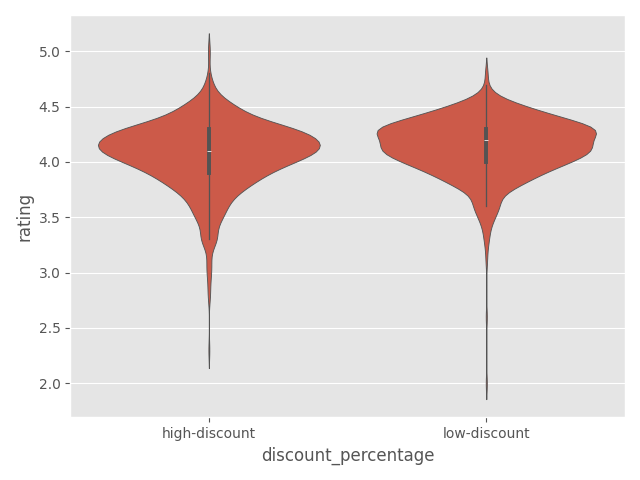
\includegraphics[width=0.8\textwidth]{./images/violin_of_rating_for_different_discount_percentages.png} % Change the filename and path
    \caption{Violin Plot of \textbf{rating} for different levels of \textbf{discount\_percentage}}
    \label{fig:Figure_6}
\end{figure}

\noindent\textbf{Distribution of rating for different price groups}:

\noindent\textbf{Analysis}: By having a look at Figure~\ref{fig:Figure_7}, we can say that different levels of \textbf{price}, namely, low, medium and high, don't seem to significantly differ in terms of \textbf{rating}. Also it looks that the distribution of all of the levels is approximately normmal. \\ 

\noindent\textbf{Relevance}: This anaylsis would be continued further, in Hypothesis Testing section, in order to examine the difference between these  three different levels of \textbf{price} in terms of \textbf{rating}. \\

\begin{figure}[H]
    \centering
    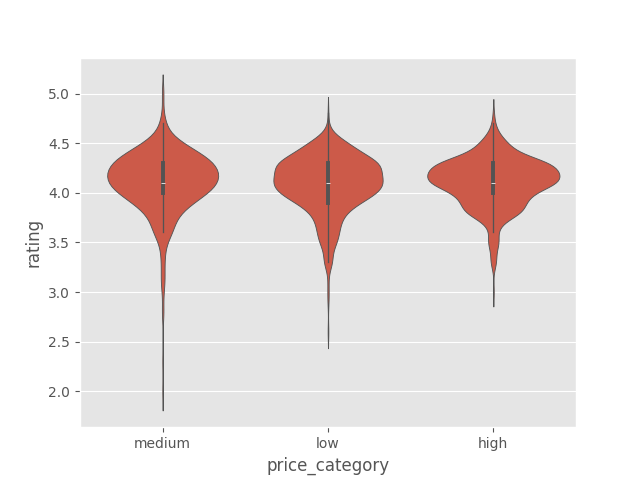
\includegraphics[width=0.8\textwidth]{./images/violinplot_of_rating_for_different_price_groups.png} % Change the filename and path
    \caption{Violin Plot of \textbf{rating} for different levels of \textbf{price}}
    \label{fig:Figure_7}
\end{figure}


\section*{Hypothesis Testing:}

\subsection*{1. Does the \textbf{discounted price} significantly impact product \textbf{ratings?}}

\noindent\textbf{Test used}: \textit{\textbf{Spearman Correlation Test}} \\ 

\noindent\textbf{Reason for why we used this test}: In our earlier analysis in Exploratory Data Analysis Section, we saw that the variables are not normally distributed. Thus the normality assumption of \textit{\textbf{Pearson Correlation Test}} is violated and we can't use it.\\

\noindent\textbf{Result}: Spearman Correlation: 0.080, P-value: 0.002\\ 

\noindent\textbf{Interpretation \& Discussion}: We both see an exteremly low p-value meaning that their is a significant monotonic relationship between these two variables as well as correlation coefficient close to zero, meaning that there isn't a relationship between these two. It seems to be a contradiction. At the end we would say that these two variables aren't correlation because it matches with out prior analysis better. \\

\subsection*{2. Are product categories and high/low ratings independent?}

\noindent\textbf{Test used}: \( \chi^2-test\).\\ 

\noindent\textbf{Result}: Chi-Squared Statistic: 213.369, P-value: 0.000. \\ 

\noindent\textbf{Interpretation \& Discussion}: We have obtained a low p-value which matches perfectly with what we saw in our prior analysis in Exploratory Data Analysis Section. Thus we accept that there is a significant dependency between these two variables. \\ 

\subsection*{3. Is there a significant difference in ratings between high-discount and low-discount products?}

\noindent\textbf{Test used}: student's two sample \( t-test \).\\ 

\noindent\textbf{Result}: T-statistic: -4.261, P-value: 0.000 \\ 

\noindent\textbf{Interpretation \& Discussion}: This result, actually is in contradiction with our prior analysis in Exploratory Data Analysis(EDA) scetion. Thus we should have a closer look at the distribution of \textbf{rating} for different levels of \textbf{discount\_percentage}. By having a look at Figure~\ref{fig:Figure_8}, we could see the difference that the hypothesis test has found(there at the picture, we could clearly see a difference that's about ~0.4) and convince ourselves that our analysis was wrong. Thus we accept a significant relationship between \textbf{discount\_percentage} and \textbf{rating}. \\ 

\begin{figure}[H]
    \centering
    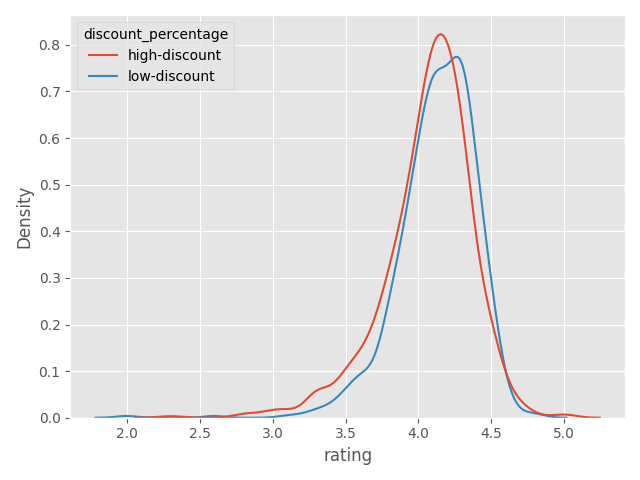
\includegraphics[width=0.8\textwidth]{./images/distro_of_rating_for_different_discount_percentages.png} % Change the filename and path
    \caption{Distribution of \textbf{rating} for different \textbf{discount\_percentage} levels}
    \label{fig:Figure_8}
\end{figure}

\subsection*{4. Do more expensive products receive higher ratings on average?}

\noindent\textbf{Test used}: ANOVA one-way test. \\ 

\noindent\textbf{Considerations}: We have used 33rd and 66th percentiles to divide the range of \textbf{price} into three different levels, namely, low, medium and high. We used this method for division because the data is skewed and this methid is robus to skewness of the data. \\ 

\noindent\textbf{Result}: F-statistic: 0.907, P-value: 0.404 \\ 

\noindent\textbf{Interpretation \& Discussion}: This matches with prior analysis from the Exploratory Data Analysis section. Thus we conclude that there isn't a significant differnece between different levels of \textbf{price} in terms of \textbf{rating}. \\ 

\subsection*{5. Does the distribution of rating counts follow a normal distribution?}

\noindent\textbf{Test used}: Shapiro-Wilk's test \\ 

\noindent\textbf{Result}: Shapiro-Wilk Test Statistic: 0.407, P-value: 0.000. \\ 

\noindent\textbf{Interpretation \& Discussion}: This tells us that \textbf{rating\_count} of distinct products is not normally distributed and it actually matches with our prior analysis in Exploratory Data Analysis section.\\ 

% \end{multicols}

\end{document}